\chapter{Introduction}\label{chap:introduction}
Robotics celebrated its 50th birthday in 2011, dating back to the first commercial robot in 1961 (the Unimate). In a ``Tonight Show'' from the time, this robot did amazing things: it opens a bottle of beer, pours it, puts a golf ball into the hole, and even conducts an orchestra. This robot does all what we expect a good robot to do: it is dexterous, it is accurate, and even creative. Since this robot's appearance on the Tonight show, more than 50 years have passed --- so how incredible must be the capabilities of today's robots and what must they be able to do?

Interestingly, we just recently learned doing all the things demonstrated by Unimate autonomously. Unimate indeed did what was shown on TV, but all motions have been preprogrammed and the environment has been carefully staged.  Only the advent of cheap and powerful sensors and computation has recently enabled robots to detect an object by themselves, plan motions to it and grasp it. Yet, robotics is still far away from doing these tasks with human-like performance.

This book introduces you to the computational fundamentals of autonomous robots. Robots are \emph{autonomous} when they make decisions in response to their environment vs.\ simply following a pre-programmed set of motions. They achieve this using techniques from signal processing, control theory, and artificial intelligence, among others. These techniques are coupled with the mechanics, the sensors, and the actuators of the robot. Designing a robot therefore requires a deep understanding of both algorithms and its interfaces to the physical world.

The goals of this introductory chapter are to introduce the kind of problems roboticists deal with and how they solve it.

\section{Intelligence and embodiment}
Our notion of ``intelligent behavior'' is strongly biased by our understanding of the brain and how computers work: intelligence is located in our heads. In fact, however, a lot of behavior that looks intelligent can be achieved by very simple means. For example, mechanical wind-up toys can avoid falling off an edge simply by using a fly-wheel that rotates at a right angle to their direction of motion and a caster wheel. Once the caster wheel loses contact with the ground---that is the robot has reached the edge---the fly-wheel kicks in and pulls the robot to the right (Figure~\ref{fig:winduptoy}).

\begin{figure}
	\centering
		\includegraphics[width=\textwidth]{figs/winduptoysketch.png}
	\caption{A wind-up toy that does not fall off the table using purely mechanical control. A fly-wheel that turns orthogonal to the robot's motion induces a right turn as soon as it hits the ground once the front caster wheel goes off the edge.}
	\label{fig:winduptoy}
\end{figure}

A robot vacuum cleaner might solve the same problem very differently: it employs infrared sensors that are pointed downwards to detect edges such as stairs and then issues a command to make an avoiding turn. Once electronics are on-board, this is a much more efficient, albeit much more complex, approach.

Whereas the above examples provide different approaches to implement intelligent behaviors, similar trade-offs exist for robotic planning. For example, ants can find the shortest path between their nest and a food source by simply choosing the trail that already has more pheromones, the chemicals ants communicate with, on it. As shorter paths have ants not only moving faster towards the food, but also returning faster, their pheromone trails build up quicker (Figure~\ref{fig:ants}). But ants are not stuck to this solution. Every now and then, ants give the longer path another shot, eventually finding new food sources. What looks like intelligent behavior at the swarm level, is essentially achieved by a pheromone sensor that occasionally fails. A modern industrial robot would solve the problem completely different: it would first acquire some representation of the environment in the form of a map populated with obstacles, and then plan a path using an algorithm.

\begin{figure}
	\centering
		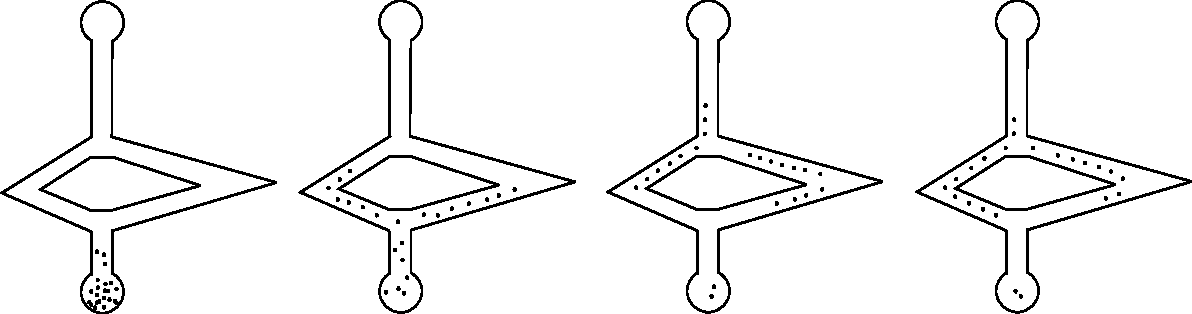
\includegraphics[width=\textwidth]{figs/ants.png}
	\caption{Ants finding the shortest path from their nest (bottom) to a food source (top). From left to right: The ants initially have equal preference for the left and the right branch, both going back and forth. As ants return faster on the shorter branch there will be more pheromones present on the short branch once a new ant arrives from the nest.}
	\label{fig:ants}
\end{figure}

Which solution to achieve a certain desired behavior is best depends on the resources that are available to the designer. We will now study a more elaborate problem for which many, more or less efficient, solutions exist.

\section{A roboticists' problem}
Imagine the following scenario. You are a robot in a maze-like environment such as a cluttered warehouse, hospital or office building. There is a chest full of gold coins hidden somewhere inside. Unfortunately, you don't have a map of the maze. In case you find the chest, you may only take a couple of coins at a time, and bring them to the exit door where your car is parked.

\begin{framed}
Think about a strategy that will allow you to harvest as many coins in the shortest time as possible. Think about the cognitive and perception capabilities you would make use of. Now discuss alternative strategies, if you would not have these capabilities, i.e., what if you were blind, had no memory?
\end{framed}

These are exactly the same problems a robot would have. A robot is a mobile machine that has sensors and computation, which allows it to reason about its environment. Current robots are far from the capabilities that humans have, therefore it makes a lot of sense to think about what strategies \emph{you} would employ to solve a problem, if you were lacking important perception or computational capabilities.

Before we move forward to discuss potential strategies for robots with impeded sensory systems, lets quickly consider an optimal strategy. You will need to explore the maze without entering any branch twice. You can use a technique known as \emph{depth-first search} to do this, but will need to be able to not only map the environment, but also localize in the environment, e.g., by recognizing places and dead-reckoning on the map. Once you have found the gold, you will need to plan the shortest path back to the exit, which you can then use to go back and forth until all the gold is harvested.

\section{Ratslife}\label{sec:ratslife}
Ratslife is a miniature robot maze competition developed by Olivier Michel from Cyberbotics S.A. The Ratslife environment can easily be created from LEGO bricks, card board or wood and the game can be played with any two mobile robots, preferably ones with the ability to identify markers in the environment. These include simple differential-wheel educational platforms with onboard cameras or even a smart-phone driven robot. Figure~\ref{fig:ratslife} shows a simple sample environment that can be constructed from craft materials and can be used to teach the practical aspects of mobile robots for competitions.


\begin{figure}
	\centering
		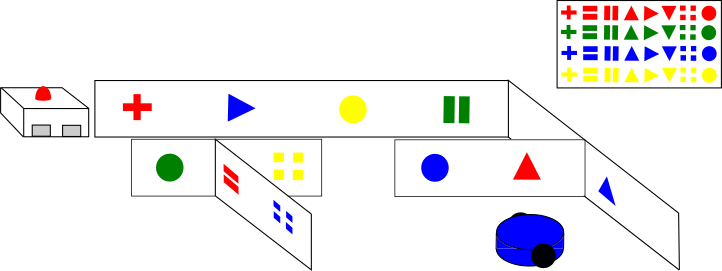
\includegraphics[width=\textwidth]{figs/ratslife.png}
	\caption{A simple maze made from cardboard, wood or Lego bricks with one or more charging stations. Locations in the maze are marked with unique markers that can be recognized by a simple robot.}
	\label{fig:ratslife}
\end{figure}



In RatsLife, two miniature robots  compete on searching for four ``feeders'' that are hidden in  a maze. Once a robot reaches a feeder, it receives ``energy'' to go on for another 60s, and the feeder becomes temporarily unavailable. After a short while, the feeder becomes available again. The feeders can be either controlled by a referee who also takes care of time-keeping or constructed as part of a simple curriculum on electronics or mechatronics.

It should be clear by now, how YOU would solve these tasks using your abilities, and you should have also thought about fall-back strategies in case some of your sensors are unavailable. Here are some possible algorithms for a robot, ordered after the capabilities that it provides:
\begin{itemize}
\item Imagine you have a robot that can only drive (actuation) and bounce off a wall. The resulting random walk will eventually let the robot reach a feeder. As the allowed time to do so is limited, it is likely that the robot's energy will soon deplete.
\item Now imagine a robot that has a sensor that gives it the ability to estimates its distance from a wall. This could be a whisker, an infrared distance sensor, an ultra-sound distance sensor, or a laser range finder. The robot could now use this sensor to keep following a wall to its right. Using this strategy for solving the maze, it will eventually explore the entire maze except for islands inside of it.
\item Finally, think about a robot that could identify simple patterns using vision, has distance sensors to avoid walls, and an ``odometer'' to keep track of its wheel rotations. Using these capabilities, a potential winning strategy would be to explore the environment, identify markers in the environment using vision and use them to create a map of all feeder locations, calculate the shortest path from feeder to feeder and keep going back and forth between them. Strategy-wise, it might make sense to wait just in front of the feeder and approach it only shortly before the robot runs out of power.
\end{itemize}

\section{Challenges of Mobile Autonomous Robots}

Being able to stitch sensor information together to map the environment just by counting your own steps and orienting yourself by using distinct features of the environment is known as Simultaneous Localization and Mapping (SLAM). The key challenge here is that the length of the steps you take are uncertain (a wheeled robot might slip or have slightly differently sized wheels, e.g.) and it is not possible to recognize places with 100\% accuracy (not even for a human). In order to be able to implement something like the last algorithm on a real robot, we will therefore need to understand

\begin{itemize}
\item How does a robot move? How does rotation of its wheels affects its position and speed in the world?
\item How do we have to control the wheel-speed in order to reach a desired position?
\item What sensors exist for a robot to perceive its own status and its environment?
\item How can we extract structured information from a vast amount of sensor data?
\item How can we localize in the world?
\item How can error be represented and how can we reason in the face of uncertainty?
\end{itemize}

In order to answer these questions, we will rely on trigonometry, linear algebra, and probability theory. Specific concepts that will be used throughout this book are basic trigonometry, matrix notation, Bayes' formula, and the concept of probability distributions. You will see that robotics is actually a great vehicle to add meaning to these concepts!


\section{Challenges of Autonomous Manipulation}
Think about the last time you worked with your hands. This includes typing on your keyboard, writing on a piece of paper, sewing a button onto a shirt, and using a hammer or a screwdriver. You will notice that these activities require a wide range of dexterity, that is the ability to manipulate objects with precision, a wide range of forces, and a wide range of sensorial capabilities. You will also notice that some tasks go beyond your capabilities, such as putting yarn through a hole in fabric, grasping a screw, or driving a nail into a piece of wood, but can be easily solved with the right tool.

So far, robotic hands are far from reaching the dexterity of a human hand. Yet, with the right tool (called ``end-effector'' in robotics speech) \index{End-effector} some tasks can be solved even better, that is faster and more precisely, than by humans. As for solving a mobile robotics problem, manipulation problems require you to think about the right mix of reasoning and mechanism design. For example, grasping tiny parts might be impossible with tweezers, but really easy when using a sucking mechanism. Or, picking up a test tube that is hardly visible with the robots' sensors can be picked up almost blindly when using a funnel-like mechanism at your end-effector. Unfortunately, these tricks will most likely limit the versatility of your robot, requiring you to think about the problem and the users's need as a whole.

%\section{The first industrial robot ``Unimate"}
%Since the introduction of the first industrial robot ``Unimate'' in 1961, the robotics industry classically consists of static manipulators that perform repetitive tasks such as welding or part placement, as well as of remote controlled machines for exploring hazardous areas. Recent advances in sensor technology and artificial intelligence are quickly enabling a new kind of robotic system: robots that can make autonomous decisions. The most prominent example of this class of robots is iRobot's ``Roomba'' vacuum cleaner that was introduced in 2002 and that uses a variation of algorithm \#1 above to solve the floor cleaning problem due to the lack of sophisticated sensors and computation. More recently, SLAM has found its ways into cars, university teams winning the DARPA Grand Challenge, Google's cars logging more than 140,000 miles, and Volkswagen presenting the first assisted driving system in 2011. Similarly, KIVA systems  successfully distributes mobile robots for automatic warehouses. These robots are still remote controlled and operate in constrained environments that provide them the ability to localize and reason on a simplified representation of the world - all items in the KIVA world are living on a grid. Novel sensors such as the xBox Kinect that provide 3D depth measurements at unprecedented low cost, increasingly capable and cheap computers, and a better understanding on how to reason about uncertainty will enable a large number of applications raising from autonomous warehouse helpers, home and elderly care, robotic toys and many other gimmicks straight from the Jetsons very soon.



\section*{Take-home lessons}
\begin{itemize}
\item How to best solve a problem is a function of the available sensing, actuation, computation and communication abilities of the available platform. Usually, there exist trade-offs that allow you to solve a problem using a minimal set of resources, but compromise performance such as speed, accuracy or reliability.
\item Robotics problems are different from problems in pure Artificial Intelligence, that do not deal with unreliable sensing or actuation.
\item The unreliability of sensors, actuators and communication links require a probabilistic notion of the system and reason with uncertainty.
\end{itemize}

\section*{Exercises}\small
\begin{enumerate}
\item What kind of sensors do you need to solve the ``Ratslife'' game? Think both about trivial and close-to-optimal approaches.
\item What devices in your home could be considered robots? Why and why not?
\item Which industries have been recently revolutionized by robotics? Into which industries were robots introduced first?
\item What sensors are you using when grasping an object? Enumerate them all. Which ones are absolutely necessary for good performance?
\item Think about robots vacuuming your floor or mowing your lawn. Do they use any planning? Why or why not?
\item What kind of sensors would you need in a car that drives completely autonomously? Think first about the kind of information that the car needs to be aware of and then discuss possible sensors that could capture this information.
\item Implement a simple line-following using a robot of your choice. How does the thickness of the line affect the sensor placement on the robot? How does its curvature affect the robot's speed?
\item Implement a maze solving algorithm that uses simple wall-following using a robot of your choice. How does the sensor geometry affect the robot's performance? What are the parameters that you find yourself tuning?
\end{enumerate}\normalsize

%Robotics celebrated its 50th birthday in 2011, dating back to the first commercial robot in 1961 (the Unimate). In a ``Tonight show'' from the time, this robot did amazing things: its opening a bottle of beer, pouring it, putting a golf ball into the hole, and even conducting an orchestra. This robot does all what we expect a good robot to do: its dexterous, its accurate, and even creative. Since this robots appearance on the Tonight show more than 50 years have passed --- so how incredible must be the capabilities of today's robots and what must they be able to do?
%
%Interestingly, we just recently learned doing all the things demonstrated by Unimate autonomously. Unimate indeed did what was shown on TV, but all motions have been pre-programmed and the environment has been carefully staged.  Only the advent of cheap and powerful sensors and computation has recently enabled robots to detect an object by themselves, plan motions to it and grasp it. Yet, robotics is still far away from doing these tasks with human-like performance. Environments still need to be heavily staged for a robot to operate, and some objects are easier to work with than others. For example, ``Rollin' Justin'' is demonstrating skills very similar to those shown by the Unimate, but is able to perceive and reason about its environment:
%
%This works as follows: the robot perceives its environment with a sensor that generates 3D range data, such as stereo-vision, a sweeping laser scanner or an xbox Kinect. The robot creates a 3D representation of its environment that is relative to its own coordinate system. The robot now plans its motion using this 3D representation. This can be seen in the inset to the top right when the robot is manipulating items on the table. Detecting objects in the environment, matching them to their 3D model, and finding feasible grasp points are still major research challenges.
%
%The ``sense-plan-act'' paradigm, that is obtaining a 3D model of the world, planning therein, and consequently executing actions is not the final solution, however. Do humans really do this when performing complex manipulations? Rather not. Instead, we are relying on vision feedback or the sense of touch when performing a grasp. (Try to grasp an object after putting your hand on an ice block, temporarily impeding your sense of touch.)
%
%This class builds up on ``Introduction to Robotics'' and introduces current solutions to these problems. We will learn advanced concepts in robotic kinematics, such as car-like steering and inverse kinematics of high-DOF manipulators, feature recognition, RGB-D perception, visual servoing and SLAM. We will also learn to use state-of-the-art tools that allow you to model, visualize and control your robot. You will work with a 7-DOF manipulator arm both in simulation and using real hardware. The development environment consists of Ubuntu Linux, ROS and OpenCV that are available as VirtualBox. The real manipulator arm is available for experimentation in the lab. We will perform laboratory experiments - that can be mostly prepared and executed in simulation - that will introduce the tools and methods we are using and guide you toward an independent project.
%
%The class consists of homework assignments (experiments) and a team project. The final deliverable for the team project is a 3 page (5 pages) for undergraduates (graduate students). Your team project needs to articulate a hypothesis (what do you want to show?) that is validated experimentally on physical hardware. In order to prepare you for this, each laboratory exercise will require analysis of experimental data rather than submission of code.
